\documentclass[9pt,t,aspectratio=169]{beamer}
\usetheme[white]{Wisconsin}
\usepackage[utf8]{inputenc}
\setbeamertemplate{page number in head/foot}[totalframenumber]
\setbeamerfont{title}{size=\LARGE}
\setbeamerfont{subtitle}{size=\Large}
\setbeamerfont{block body}{size=\footnotesize}
\setbeamerfont{author}{size=\LARGE}
\setbeamerfont{date}{size=\Large}
\setbeamerfont{institute}{size=\large}
\setlength{\leftmargini}{0pt}

%subcaptions
\usepackage{subcaption}
% \captionsetup[subfigure]{labelformat=empty} % turn off labeling figures

% turn off Figure in captions
\usepackage{caption}
% \captionsetup[figure]{labelformat=empty}

\newcommand{\QOR}{\qquad \text{OR} \qquad}
\newcommand{\QAND}{\qquad \text{AND} \qquad}
\newcommand{\QTHUS}{\qquad \text{THUS} \qquad}
\newcommand{\QTHEN}{\qquad \text{THEN} \qquad}
\newcommand{\QWITH}{\qquad \text{WITH} \qquad}
\newcommand{\QFOR}{\qquad \text{FOR} \qquad}
\newcommand{\QSO}{\qquad \text{SO} \qquad}
\newcommand{\QWHERE}{\qquad \text{WHERE} \qquad}
\newcommand{\LINE}{\par\noindent\rule{\textwidth}{0.4pt}\par}
\newcommand{\toinf}{\rightarrow\infty}
\newcommand{\tozero}{\rightarrow0}
\newcommand{\qeq}{\overset{?}{=}}
\newcommand{\ceq}{\overset{\checkmark}{=}}
\renewcommand{\epsilon}{\varepsilon}
\newcommand{\keff}{$k_{e\!f\!f}$}


% table packages
\usepackage{booktabs}

% Roman Numerals
\newcommand{\rom}[1]{\expandafter\uppercase{\Romannumeral #1\relax}}

% hypersetup
\usepackage{hyperref}
\hypersetup{colorlinks,
            linkcolor = black,
            citecolor = black,
            urlcolor = cyan
}


\def\brac#1{\{#1\}}
\def\Brac#1{\big\{#1\big\}}
\def\BRAC#1{\bigg\{#1\bigg\}}
\def\angbrac#1{\langle#1\rangle}
\def\Angbrac#1{\big\langle#1\big\rangle}
\def\ANGBRAC#1{\bigg\langle#1\bigg\rangle}

% % Transitional slides between sections
% \AtBeginSection[]
% {
%     \begin{frame}
%         \frametitle{Table of Contents}
%         \tableofcontents[currentsection]
%     \end{frame}
% }


% Bibliography
\usepackage[sorting=none]{biblatex} %Imports biblatex package and cites in order of appearance
\addbibresource{physor2024_pres.bib} %Import the bibliography file
% make all font colors white
\setbeamercolor{bibliography item}{fg=black}
\setbeamercolor{bibliography entry author}{fg=black}
\setbeamercolor{bibliography entry title}{fg=black}
\setbeamercolor{bibliography entry location}{fg=black}
\setbeamercolor{bibliography entry note}{fg=black}
% adds numeric labels linked to bib entries
\setbeamertemplate{bibliography item}{\insertbiblabel}

% eliminate header within an environment
\makeatletter
    \newenvironment{withoutheadline}{
       \setbeamertemplate{headline}[default]
       \def\beamer@entrycode{\vspace*{-\headheight}}
    }{}
\makeatother

% appendix renumbering
\usepackage{appendixnumberbeamer}
% frame breaks with same title
\setbeamertemplate{frametitle continuation}[from second][]

\title{Exploring Effects of Homogenization on an OpenMC Depletion Analysis}
\subtitle{of a TRISO Fueled, Helium Cooled Microreactor}
\author{\vspace*{-0.45cm}Lewis I. Gross\textsuperscript{1}, Patrick Shriwise\textsuperscript{2,1}, Benjamin Lindley\textsuperscript{1} and Paul P.H. Wilson\textsuperscript{1}}
\institute{University of Wisconsin-Madison\textsuperscript{1}, Argonne National Lab\textsuperscript{2} }
\date{\vspace*{-0.25cm}April 24, 2024}
%%----------------------------------------------------------------------------%%
\begin{document}

\begin{withoutheadline}
\begin{frame}[plain] % the plain makes the first frame look good
    \maketitle
\end{frame}
\end{withoutheadline}

\author{Lewis Gross, Patrick Shriwise, Ben Lindley, and Paul Wilson} % reset author so affiliations don't show up in footer
%%----------------------------------------------------------------------------%%
%% Overview
%%----------------------------------------------------------------------------%%
\begin{withoutheadline}
\begin{frame}{Outline}
  \tableofcontents
\end{frame}
\end{withoutheadline}


%%----------------------------------------------------------------------------%%
%% Section 1
%%----------------------------------------------------------------------------%%
\section{Virtual Test Bed Gas-Cooled Microreactor}
\hypersetup{citecolor=white}
\begin{frame}{Microreactors \cite{INL_MR}}
    \begin{figure}
        \centering
        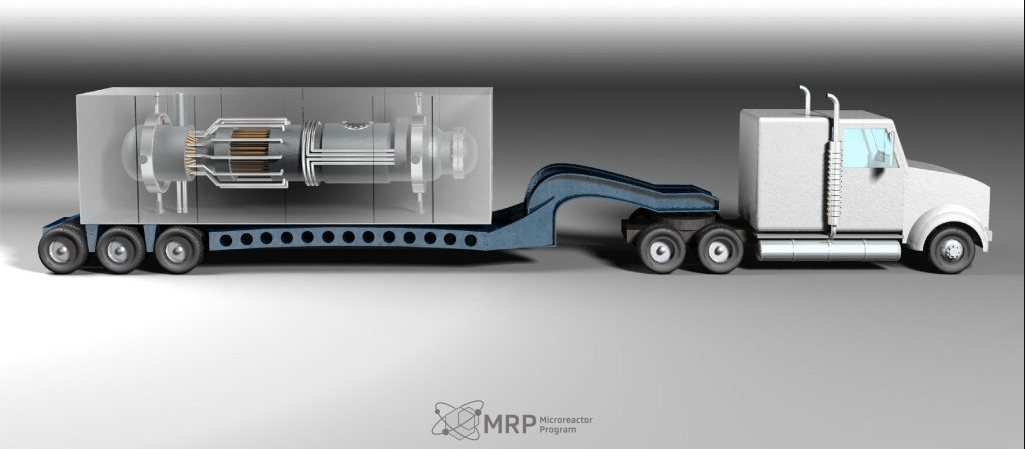
\includegraphics[width=0.95\linewidth]{figures/INL_MR.png}
    \end{figure}
\end{frame}

\begin{frame}{Virtual Test Bed \cite{vtb2023}}
    \begin{figure}
        \centering
        
\includegraphics[width=0.6\linewidth]{figures/nric_logo.png}
    \end{figure}
    \begin{figure}
        \centering
        
\includegraphics[width=0.6\linewidth]{figures/NEAMS.png}
    \end{figure}
\end{frame}
\hypersetup{citecolor=black}

\begin{frame}{Virtual Test Bed Gas Cooled Microreactor}
    \begin{itemize}
        \item Existing work/simulations
        \item First OpenMC Model of the VTB GCMR, plans to add this model to the VTB this summer
        \item TRISO modeling challenges
    \end{itemize}
\end{frame}

\begin{frame}{Goal of this work}
    \begin{itemize}
        \item
    \end{itemize}
\end{frame}

%%----------------------------------------------------------------------------%%
%% Section 2
%%----------------------------------------------------------------------------%%
\section{OpenMC Model}

\begin{frame}{TRISO particles}
    \begin{itemize}
        \item Image showing the explicit TRISO and packing into fuel compact
        \item Image showing the kernel only
        \item Explain how the homogenization works (total fuel atoms preserved)
    \end{itemize}
\end{frame}

\begin{frame}{Slice Plots}
    \begin{figure}
        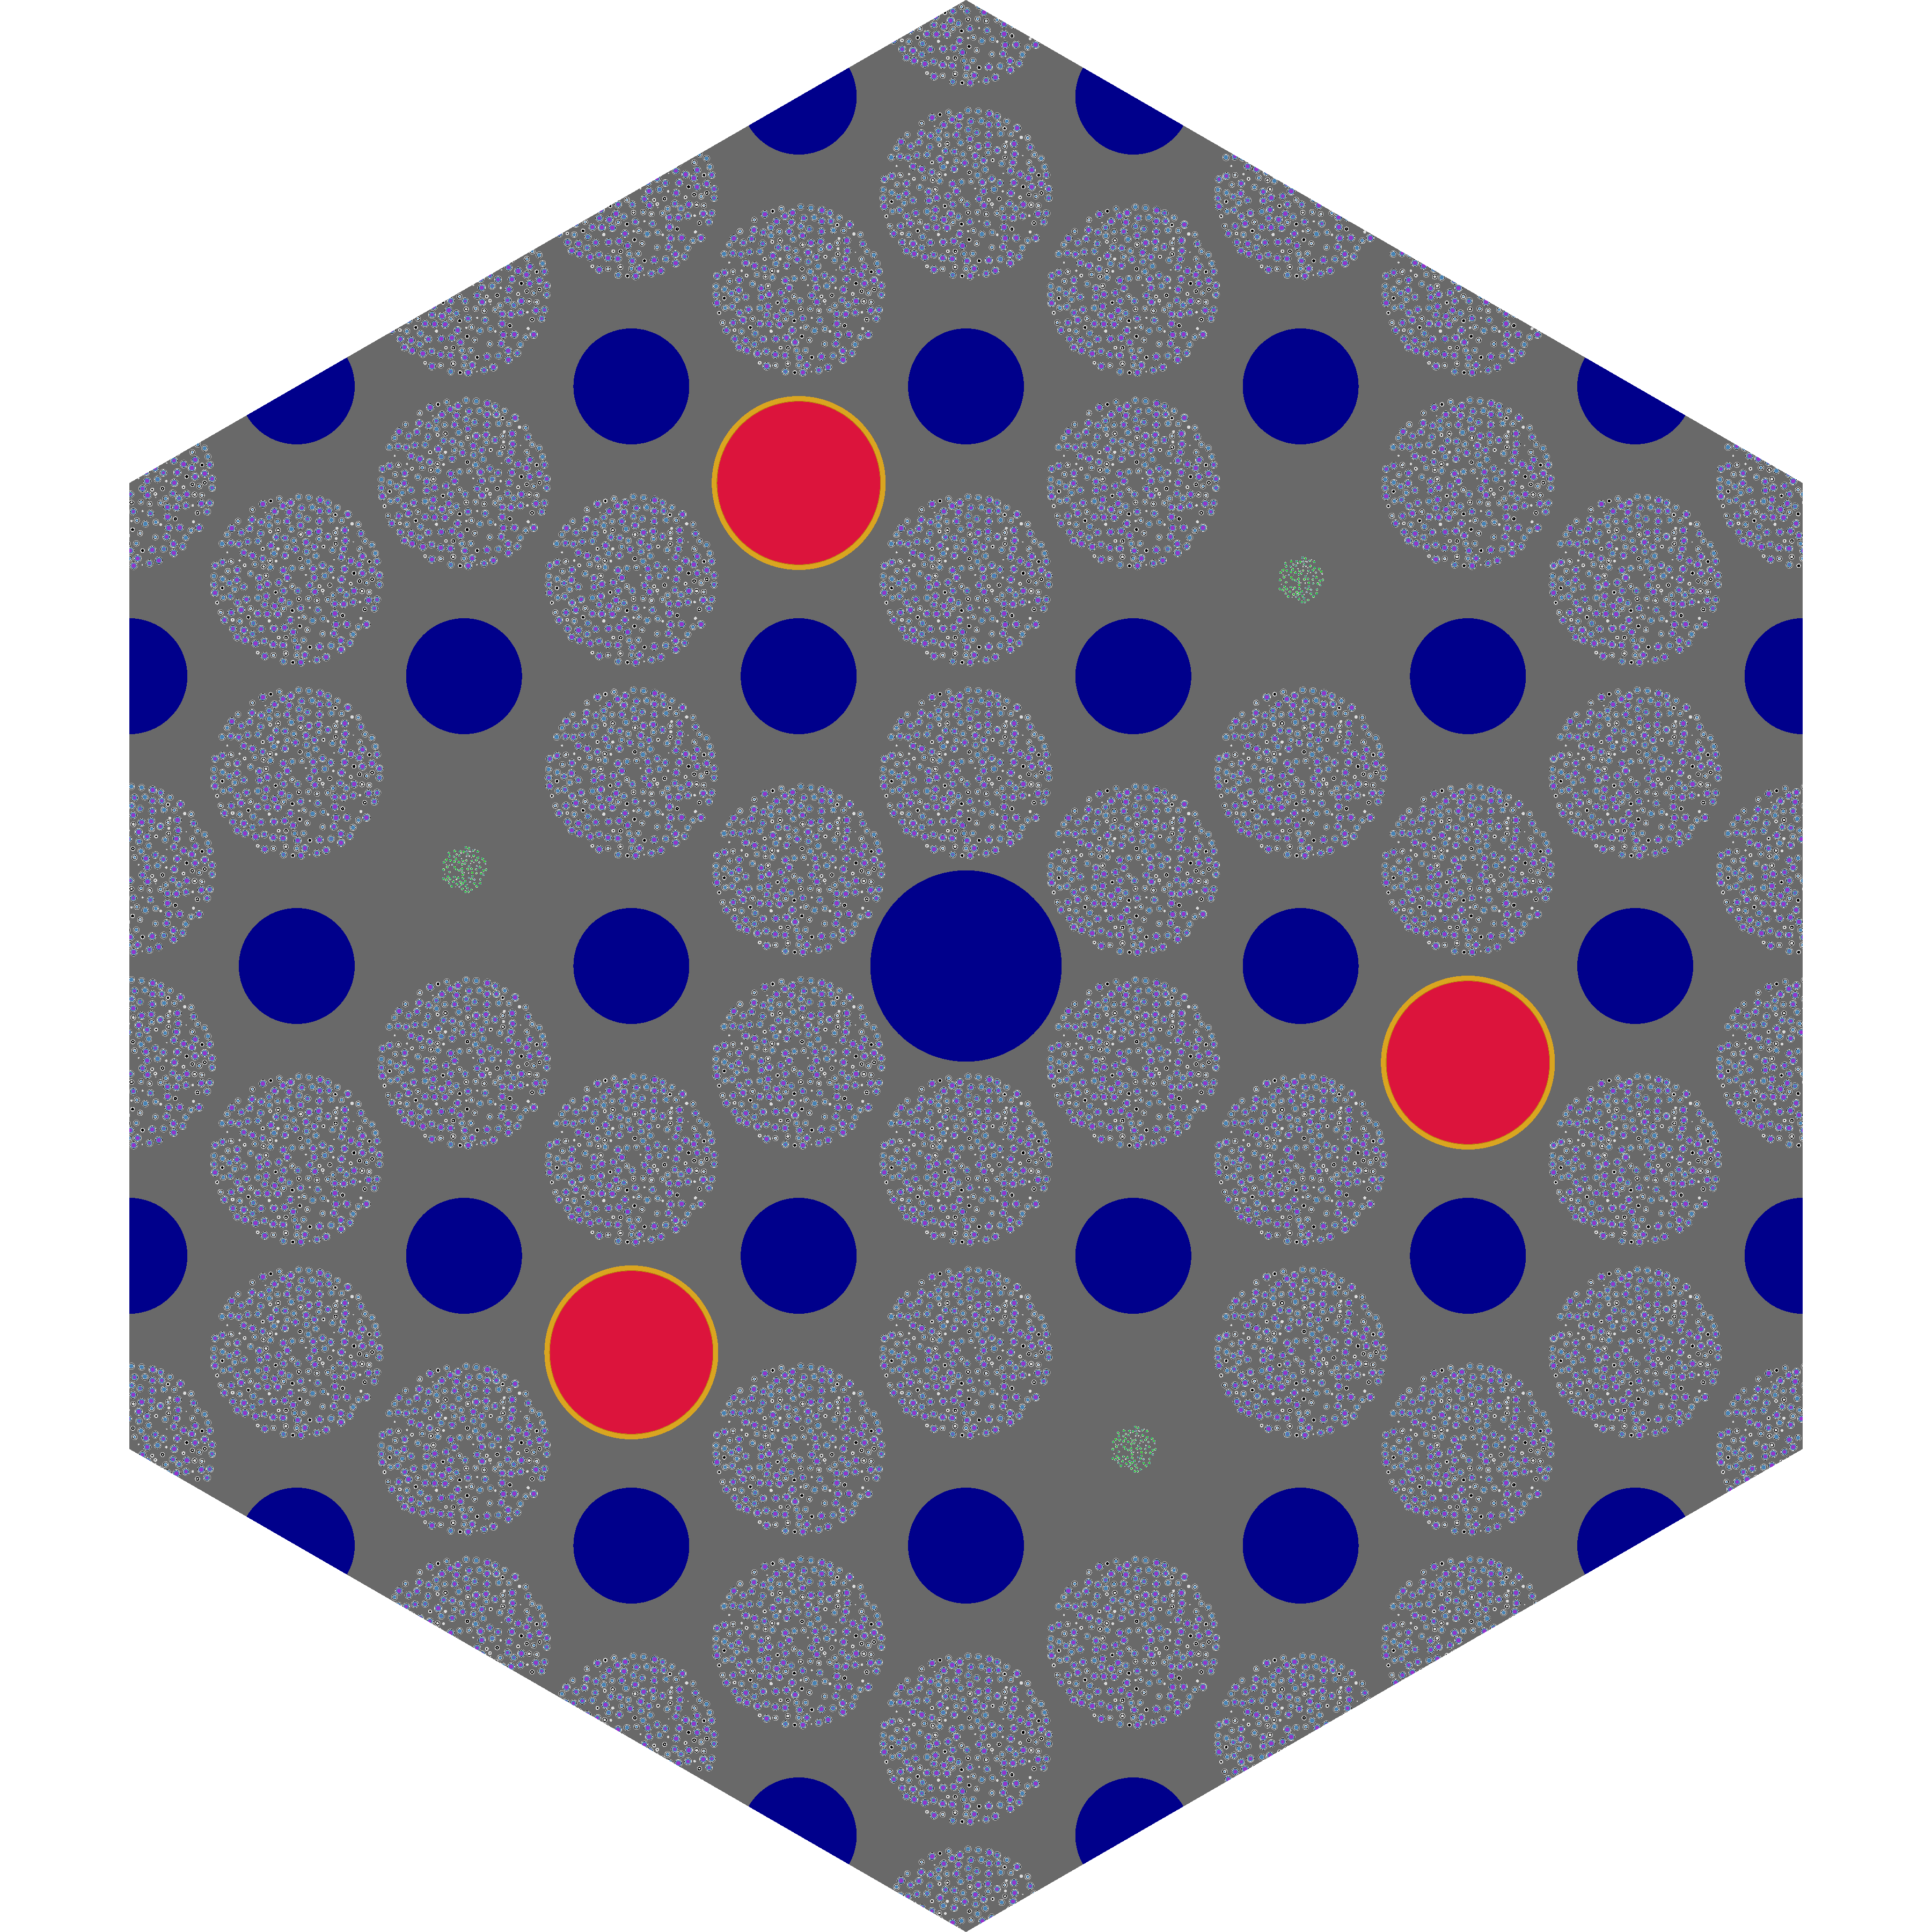
\includegraphics[height=0.8\textheight]{figures/gcmr_slice.png}
    \end{figure}
\end{frame}


\begin{frame}{Depletion Simulation Definitions}
    \begin{itemize}
        \item
    \end{itemize}
\end{frame}

%%----------------------------------------------------------------------------%%
%% Section 3
%%----------------------------------------------------------------------------%%
\section{Results and Discussion}

\begin{frame}{Eigenvalue comparisons across each spatial discretization}
    \begin{itemize}
        \item ratios vs burnup
    \end{itemize}
\end{frame}

\begin{frame}{Eigenvalue comparisons across each spatial discretization}
    \begin{itemize}
        \item average delta rhos
    \end{itemize}
\end{frame}

\begin{frame}{Eigenvalue comparisons across each spatial discretization}
    \begin{itemize}
        \item isotopics
    \end{itemize}
\end{frame}

%%----------------------------------------------------------------------------%%
%% Section 4
%%----------------------------------------------------------------------------%%
\section{Next Steps}
\begin{frame}{Two-layer TRISO Homogenization}
    \begin{itemize}
        \item
    \end{itemize}
\end{frame}

\begin{frame}{Full core model and multiphysics}
    \begin{itemize}
        \item
    \end{itemize}
\end{frame}


%%----------------------------------------------------------------------------%%`'
%% Bibliography
%%----------------------------------------------------------------------------%%

\begin{withoutheadline}
    \begin{frame}{Acknowledgements}
        \begin{itemize}
            \item The first author was supported in part by the US Nuclear Regulatory Commission's Graduate Fellowship Program administered by the University of Wisconsin-Madison.
            \item The Center for High Throughput Computing at the University of Wisconsin - Madison
            \item OpenMC team!
            \item Co-authors: Patrick Shriwise, Benjamin Lindley and Paul P.H.~Wilson.
        \end{itemize}
        \begin{figure}[H]
            \centering
            
\includegraphics[height=0.3\textheight]{figures/openmc_logo.png}
        \end{figure}
        \begin{figure}[H]
            \centering
            
\includegraphics[height=0.3\textheight]{figures/CHTC.png}
        \end{figure}
    \end{frame}
\end{withoutheadline}

\begin{withoutheadline}
    \begin{frame}[allowframebreaks]{Bibliography}
        \printbibliography
    \end{frame}
\end{withoutheadline}

\begin{withoutheadline}
    \begin{frame}{Open Source Projects}
        \begin{itemize}
            \item OpenMC website: \href{https://openmc.org/}{https://openmc.org/}
            \item OpenMC repository: \href{https://github.com/openmc-dev/openmc}{https://github.com/openmc-dev/openmc}
            \item VTB: \href{https://mooseframework.inl.gov/virtual_test_bed/}{https://mooseframework.inl.gov/virtual\_test\_bed/}
            \item VTB repository: \href{https://github.com/idaholab/virtual_test_bed}{https://github.com/idaholab/virtual\_test\_bed}
            \item Add me on LinkedIn (\href{https://www.linkedin.com/in/lewisgross1296}{lewisgross1296}) and GitHub (\href{https://github.com/lewisgross1296}{lewisgross1296})!
        \end{itemize}
    \end{frame}
\end{withoutheadline}

\end{document}
